\documentclass{standalone}
\usepackage{tikz}
\usetikzlibrary{patterns, positioning}

\begin{document}
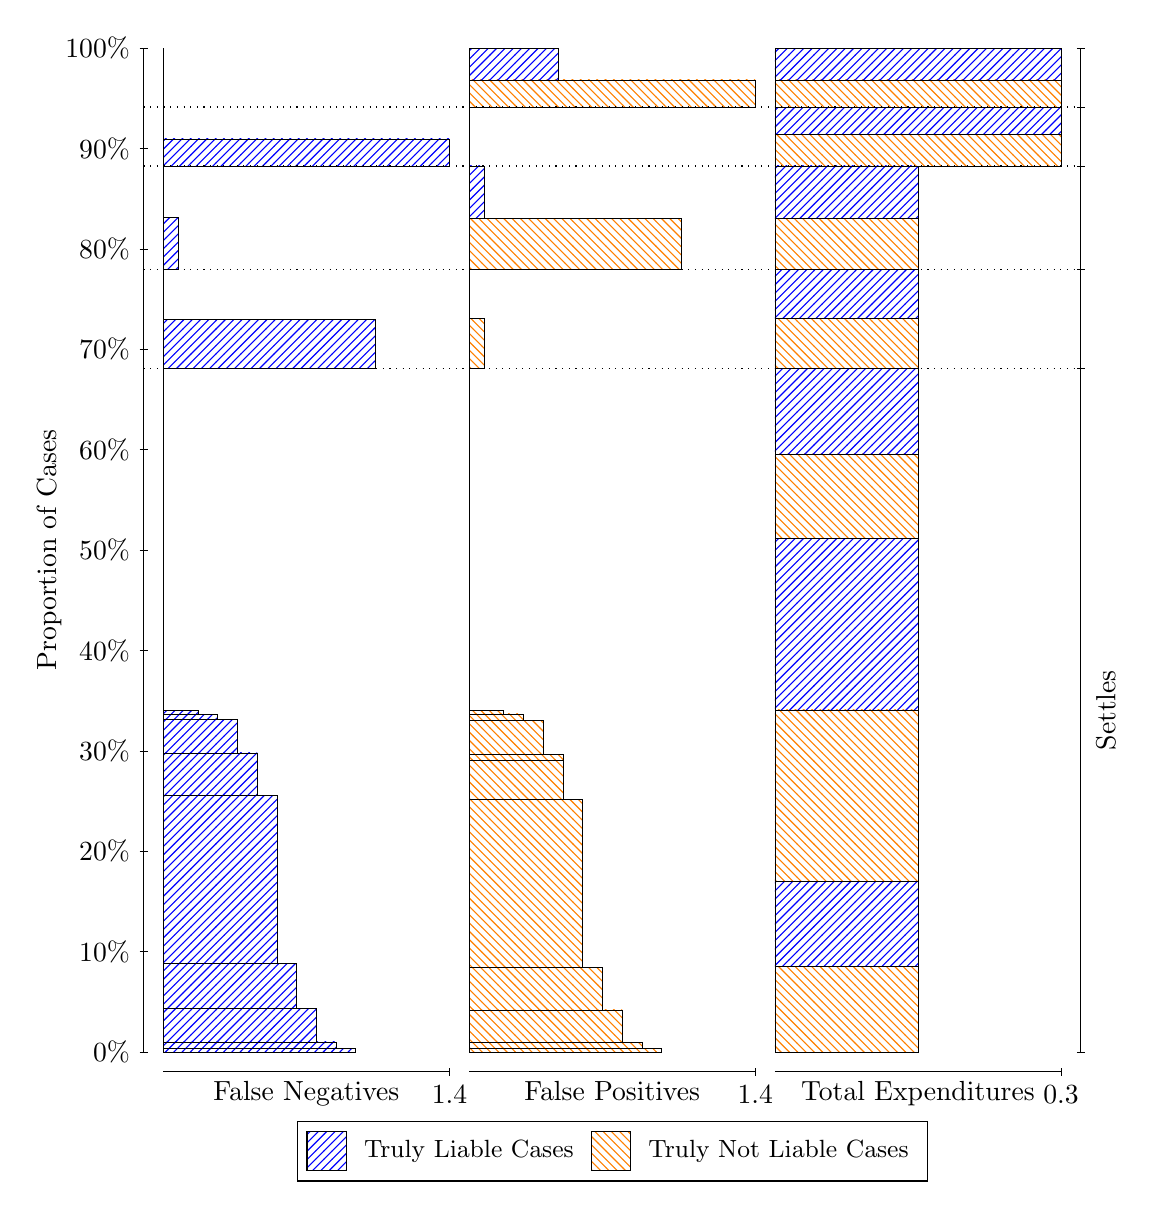
\begin{tikzpicture}
\draw[black, very thin] (1.5,1.75) -- (1.5,14.5);
\node[rotate=90, anchor=center] at (0.3, 8.125) {Proportion of Cases};
\draw[black, very thin] (1.45,1.75) -- (1.55,1.75);
\node[anchor=east] at (1.45, 1.75) {0\%};
\draw[black, very thin] (1.45,3.025) -- (1.55,3.025);
\node[anchor=east] at (1.45, 3.025) {10\%};
\draw[black, very thin] (1.45,4.3) -- (1.55,4.3);
\node[anchor=east] at (1.45, 4.3) {20\%};
\draw[black, very thin] (1.45,5.575) -- (1.55,5.575);
\node[anchor=east] at (1.45, 5.575) {30\%};
\draw[black, very thin] (1.45,6.85) -- (1.55,6.85);
\node[anchor=east] at (1.45, 6.85) {40\%};
\draw[black, very thin] (1.45,8.125) -- (1.55,8.125);
\node[anchor=east] at (1.45, 8.125) {50\%};
\draw[black, very thin] (1.45,9.4) -- (1.55,9.4);
\node[anchor=east] at (1.45, 9.4) {60\%};
\draw[black, very thin] (1.45,10.675) -- (1.55,10.675);
\node[anchor=east] at (1.45, 10.675) {70\%};
\draw[black, very thin] (1.45,11.95) -- (1.55,11.95);
\node[anchor=east] at (1.45, 11.95) {80\%};
\draw[black, very thin] (1.45,13.225) -- (1.55,13.225);
\node[anchor=east] at (1.45, 13.225) {90\%};
\draw[black, very thin] (1.45,14.5) -- (1.55,14.5);
\node[anchor=east] at (1.45, 14.5) {100\%};

\draw[black, very thin] (13.4,1.75) -- (13.4,14.5);
\draw[black, very thin] (13.35,1.75) -- (13.45,1.75);
\node[anchor=west] at (13.35, 1.75) {};
\draw[black, very thin] (13.35,10.43) -- (13.45,10.43);
\node[anchor=west] at (13.35, 10.43) {};
\draw[black, very thin] (13.35,11.687) -- (13.45,11.687);
\node[anchor=west] at (13.35, 11.687) {};
\draw[black, very thin] (13.35,13.002) -- (13.45,13.002);
\node[anchor=west] at (13.35, 13.002) {};
\draw[black, very thin] (13.35,13.751) -- (13.45,13.751);
\node[anchor=west] at (13.35, 13.751) {};
\draw[black, very thin] (13.35,14.5) -- (13.45,14.5);
\node[anchor=west] at (13.35, 14.5) {};

\draw[black, very thin, pattern color=blue, pattern=north east lines] (1.75,1.75) rectangle (4.1931,1.7984);
\draw[black, very thin, pattern color=blue, pattern=north east lines] (1.75,1.7984) rectangle (3.9425,1.8774);
\draw[black, very thin, pattern color=blue, pattern=north east lines] (1.75,1.8774) rectangle (3.692,2.3077);
\draw[black, very thin, pattern color=blue, pattern=north east lines] (1.75,2.3077) rectangle (3.4414,2.8766);
\draw[black, very thin, pattern color=blue, pattern=north east lines] (1.75,2.8766) rectangle (3.1908,5.0049);
\draw[black, very thin, pattern color=blue, pattern=north east lines] (1.75,5.0049) rectangle (2.9402,5.5494);
\draw[black, very thin, pattern color=blue, pattern=north east lines] (1.75,5.5494) rectangle (2.6897,5.97);
\draw[black, very thin, pattern color=blue, pattern=north east lines] (1.75,5.97) rectangle (2.4391,6.0409);
\draw[black, very thin, pattern color=blue, pattern=north east lines] (1.75,6.0409) rectangle (2.1885,6.0886);
\draw[black, very thin, pattern color=orange, pattern=north west lines] (1.75,6.0886) rectangle (1.75,10.43);
\draw[black, very thin, pattern color=blue, pattern=north east lines] (1.75,10.43) rectangle (4.4437,11.052);
\draw[black, very thin, pattern color=orange, pattern=north west lines] (1.75,11.052) rectangle (1.75,11.687);
\draw[black, very thin, pattern color=blue, pattern=north east lines] (1.75,11.687) rectangle (1.9379,12.351);
\draw[black, very thin, pattern color=orange, pattern=north west lines] (1.75,12.351) rectangle (1.75,13.002);
\draw[black, very thin, pattern color=blue, pattern=north east lines] (1.75,13.002) rectangle (5.3833,13.346);
\draw[black, very thin, pattern color=orange, pattern=north west lines] (1.75,13.346) rectangle (1.75,13.751);
\draw[black, very thin, pattern color=orange, pattern=north west lines] (1.75,13.751) rectangle (1.75,14.095);
\draw[black, very thin, pattern color=blue, pattern=north east lines] (1.75,14.095) rectangle (1.75,14.5);
\draw[black, very thin, pattern color=orange, pattern=north west lines] (5.6333,1.75) rectangle (8.0764,1.7976);
\draw[black, very thin, pattern color=orange, pattern=north west lines] (5.6333,1.7976) rectangle (7.8259,1.8682);
\draw[black, very thin, pattern color=orange, pattern=north west lines] (5.6333,1.8682) rectangle (7.5753,2.2849);
\draw[black, very thin, pattern color=orange, pattern=north west lines] (5.6333,2.2849) rectangle (7.3247,2.8265);
\draw[black, very thin, pattern color=orange, pattern=north west lines] (5.6333,2.8265) rectangle (7.0741,4.9563);
\draw[black, very thin, pattern color=orange, pattern=north west lines] (5.6333,4.9563) rectangle (6.8236,5.4597);
\draw[black, very thin, pattern color=orange, pattern=north west lines] (5.6333,5.4597) rectangle (6.8236,5.5308);
\draw[black, very thin, pattern color=orange, pattern=north west lines] (5.6333,5.5308) rectangle (6.573,5.9643);
\draw[black, very thin, pattern color=orange, pattern=north west lines] (5.6333,5.9643) rectangle (6.3224,6.0432);
\draw[black, very thin, pattern color=orange, pattern=north west lines] (5.6333,6.0432) rectangle (6.0718,6.0915);
\draw[black, very thin, pattern color=blue, pattern=north east lines] (5.6333,6.0915) rectangle (5.6333,10.43);
\draw[black, very thin, pattern color=orange, pattern=north west lines] (5.6333,10.43) rectangle (5.8213,11.064);
\draw[black, very thin, pattern color=blue, pattern=north east lines] (5.6333,11.064) rectangle (5.6333,11.687);
\draw[black, very thin, pattern color=orange, pattern=north west lines] (5.6333,11.687) rectangle (8.327,12.338);
\draw[black, very thin, pattern color=blue, pattern=north east lines] (5.6333,12.338) rectangle (5.8213,13.002);
\draw[black, very thin, pattern color=orange, pattern=north west lines] (5.6333,13.002) rectangle (5.6333,13.406);
\draw[black, very thin, pattern color=blue, pattern=north east lines] (5.6333,13.406) rectangle (5.6333,13.751);
\draw[black, very thin, pattern color=orange, pattern=north west lines] (5.6333,13.751) rectangle (9.2667,14.095);
\draw[black, very thin, pattern color=blue, pattern=north east lines] (5.6333,14.095) rectangle (6.7609,14.5);
\draw[black, very thin, pattern color=orange, pattern=north west lines] (9.5167,1.75) rectangle (11.333,2.8369);
\draw[black, very thin, pattern color=blue, pattern=north east lines] (9.5167,2.8369) rectangle (11.333,3.9151);
\draw[black, very thin, pattern color=orange, pattern=north west lines] (9.5167,3.9151) rectangle (11.333,6.0931);
\draw[black, very thin, pattern color=blue, pattern=north east lines] (9.5167,6.0931) rectangle (11.333,8.27);
\draw[black, very thin, pattern color=orange, pattern=north west lines] (9.5167,8.27) rectangle (11.333,9.3464);
\draw[black, very thin, pattern color=blue, pattern=north east lines] (9.5167,9.3464) rectangle (11.333,10.43);
\draw[black, very thin, pattern color=orange, pattern=north west lines] (9.5167,10.43) rectangle (11.333,11.064);
\draw[black, very thin, pattern color=blue, pattern=north east lines] (9.5167,11.064) rectangle (11.333,11.687);
\draw[black, very thin, pattern color=orange, pattern=north west lines] (9.5167,11.687) rectangle (11.333,12.338);
\draw[black, very thin, pattern color=blue, pattern=north east lines] (9.5167,12.338) rectangle (11.333,13.002);
\draw[black, very thin, pattern color=orange, pattern=north west lines] (9.5167,13.002) rectangle (13.15,13.406);
\draw[black, very thin, pattern color=blue, pattern=north east lines] (9.5167,13.406) rectangle (13.15,13.751);
\draw[black, very thin, pattern color=orange, pattern=north west lines] (9.5167,13.751) rectangle (13.15,14.095);
\draw[black, very thin, pattern color=blue, pattern=north east lines] (9.5167,14.095) rectangle (13.15,14.5);
\draw[black, dotted] (1.5,10.43) -- (13.4,10.43);
\draw[black, dotted] (1.5,11.687) -- (13.4,11.687);
\draw[black, dotted] (1.5,13.002) -- (13.4,13.002);
\draw[black, dotted] (1.5,13.751) -- (13.4,13.751);
\draw[black, very thin] (1.75,1.5) -- (5.3833,1.5);
\node[anchor=north] at (3.5667, 1.5) {False Negatives};
\draw[black, very thin] (5.3833,1.45) -- (5.3833,1.55);
\node[anchor=north] at (5.3833, 1.45) {1.4};

\draw[black, very thin] (5.6333,1.5) -- (9.2667,1.5);
\node[anchor=north] at (7.45, 1.5) {False Positives};
\draw[black, very thin] (9.2667,1.45) -- (9.2667,1.55);
\node[anchor=north] at (9.2667, 1.45) {1.4};

\draw[black, very thin] (9.5167,1.5) -- (13.15,1.5);
\node[anchor=north] at (11.333, 1.5) {Total Expenditures};
\draw[black, very thin] (13.15,1.45) -- (13.15,1.55);
\node[anchor=north] at (13.15, 1.45) {0.3};

\node[black, centered, rotate=90] at (13.72, 6.09) {Settles};





\draw (7.449999999999999,1.5) node[draw=none] (baseCoordinate) {};
\begin{scope}[align=center]
        \matrix[scale=0.5, draw=black, below=0.5cm of baseCoordinate, nodes={draw}, column sep=0.1cm]{
            \node[rectangle, draw, minimum width=0.5cm, minimum height=0.5cm, pattern=north east lines, pattern color=blue] {}; &
            \node[draw=none, font=\small] (B) {Truly Liable Cases}; &
            \node[rectangle, draw, minimum width=0.5cm, minimum height=0.5cm, pattern=north west lines, pattern color=orange] {}; &
            \node[draw=none, font=\small] (B) {Truly Not Liable Cases}; \\
            };
\end{scope}

\end{tikzpicture}
\end{document}